\chapter{Related Work} \label{chap:Chapter3}       
\epigraph{``This is where technology is now, imagine where we can go in the future” }{\textit{Timothy Chung}}

Σε αυτό το \emph{Chapter} περιγράφονται τρόποι - από την βιβλιογραφία - με τους οποίους, οι υπάρχουσες εφαρμογές 
από drone swarms επιλύουν το localization problem. Κάποια από τα συστήματα στην υπάρχουσα βιβλιογραφία έχουν καθαρά
θεωρητική πλευρά, άλλα έχουν δοκιμαστεί σε real-life scenarios.
Τέλος, σε αρκετές από αυτές τις εφαρμογές χρησιμοποιούνται, 
και γίνεται αναφορά των τεχνικών που αναφέρθηκαν στο \emph{Chapter} \ref{chap:Chapter2}.



% ------------------------------------------------------------------------------------
\section{UWB, IMU and GPS}
Πρώτη αναφορά \cite{uwb-imu-gps1} \cite{uwb-imu-gps2} \cite{uwb-imu-gps3}
Ultra-Wideband Based Pose Estimation for SmallUnmanned Aerial Vehicles

Cooperative 3-D relative localization for UAV swarm by fusing UWB withIMU and GPS

Accurate  3D  Localization  for  MAV  Swarms  by  UWB  and  IMU  Fusion

\begin{figure} [H]
	\centering
	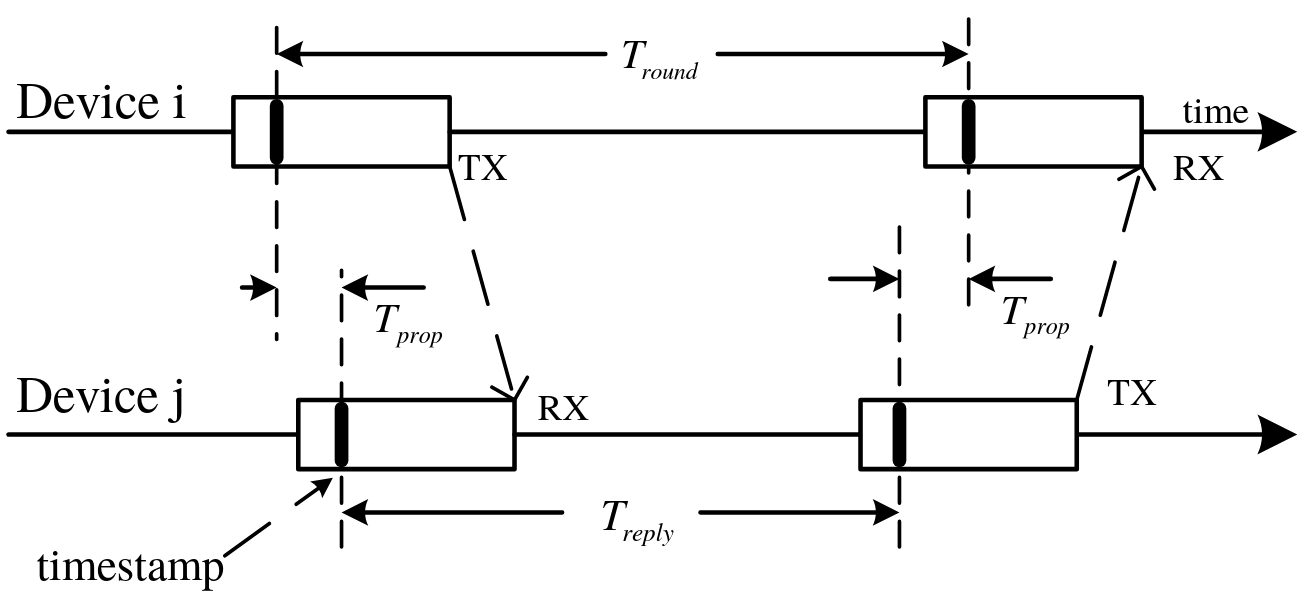
\includegraphics[width=0.7\linewidth]{Images/Related-Work/Single-Sided-Two-Way-Ranging-SS-TWR-5.png}
	\decoRule
	\caption[Illustration of Single-sided Two-way ranging]{Illustration of Single-sided Two-way ranging \cite{uwb-imu-gps1}}
	\label{fig:SS-TWR}
\end{figure}

Για κάθε node i σε συγκεκριμένο time-stamp k 
\begin{gather*}
	\textbf{GPS Position:}\quad r^k_{i, GPS} = \left[x^k_{i, GPS} \quad y^k_{i, GPS} \quad z^k_{i, GPS}\right]^T \\
	\textbf{Velocity estimation:}\quad\hat{v}^k_i = \left[\hat{v}^k_{xi} \quad \hat{v}^k_{yi} \quad \hat{v}^k_{zi}\right]^T \\
	\textbf{Acceleration estimation:}\quad\hat{a}^k_i = \left[\hat{a}^k_{xi} \quad \hat{a}^k_{yi} \quad \hat{a}^k_{zi}\right]^T
\end{gather*}

\begin{gather*}
    d_{ij} = \frac{1}{2}(T_{round} - T_{reply}) \times c = \norm{r_i - r_j} + n_{UWB}, \quad with \quad n_{UWB} \sim N(0, \sigma^2_{UWB}) 
\end{gather*}

\begin{gather*}
    r_{i,j} = r_{i, GPS} - r_{j, GPS} = r_{ij} + n_{GPS}
\end{gather*}

% \begin{gather}
        
% \end{gather}

% \begin{gather}
        
% \end{gather}


% Some systems have been deployed and tested in real-life scenarios, while others remain theoretical approaches
% \cite{10.5555/3400306.3400339}
% \cite{6907551}
% \cite{8355093}
% \cite{PMID:33348720}
% \cite{article5}
% \cite{inproceedings}
% \cite{inproceedings2}
% \cite{8453331}
% \cite{4967999}
% \cite{inproceedings51}
% \cite{trilateration-application1}
% \cite{Qi_2020}


% \section{Demo: In-flight Localisation of Micro-UAVs using Ultra-Wide Band}

% IEEE 802.15.4-2011 

% distance measurement with a precision down to 10 cm within
% a 250 m range

% It combines good obstacle penetration, and
% resilience to both multi-path effects and interference from
% other wireless technologies
% Symmetrical Double-
% Sided Two-Way Ranging 

% Local Positioning System (LPS) 




% This should be the last section
\section{Thesis Approach}
TODO: As last section of this chapter
